%=========================================================
% SEMINAR REPORT
% GENERATIVE AGENTS IN AGENT-BASED MODELING:
% OVERVIEW, VALIDATION AND EMERGING CHALLENGES
%=========================================================

\documentclass[12pt,a4paper]{report}
\usepackage[T1]{fontenc}
\usepackage[utf8]{inputenc}

%=========================================================
% PACKAGES
%=========================================================

\usepackage[a4paper,
            top=1in,
            bottom=1in,
            left=1.3in,
            right=1in]{geometry}

% PDFLaTeX-compatible Times-style font
\usepackage{newtxtext}
\usepackage{newtxmath}

\usepackage{graphicx}
\graphicspath{{./}{./figures/}}
\usepackage{fancyhdr}
\usepackage{titlesec}
\usepackage{tocloft}
\usepackage{setspace}
\usepackage{amsmath,amssymb}
\usepackage{enumitem}
\usepackage{hyperref}
\usepackage{booktabs}
\usepackage{array}
\usepackage{caption}
\usepackage{xcolor}
\usepackage{float}
\usepackage{ragged2e}
\usepackage[nottoc,notlot,notlof]{tocbibind}
\usepackage{chngcntr}
\usepackage{tabularx}
\usepackage{longtable}
\usepackage{colortbl}

%=========================================================
% HYPERLINK SETTINGS
%=========================================================

\hypersetup{
    colorlinks=true,
    linkcolor=black,
    citecolor=black,
    urlcolor=blue,
    pdftitle={GENERATIVE AGENTS IN AGENT-BASED MODELING: OVERVIEW, VALIDATION AND EMERGING CHALLENGES},
    pdfauthor={Aravind A Kamath}
}

%=========================================================
% GENERAL FORMATTING
%=========================================================

\onehalfspacing
\fontsize{12}{18}\selectfont

\setlength{\parindent}{0.5in}
\setlength{\parskip}{0pt}

%=========================================================
% CHAPTER AND HEADING NUMBERING (ARABIC 1, 2, 3)
%=========================================================

\counterwithout{figure}{chapter}
\counterwithout{table}{chapter}

\renewcommand{\thechapter}{\arabic{chapter}}
\renewcommand{\thesection}{\thechapter.\arabic{section}}
\renewcommand{\thesubsection}{\thesection.\arabic{subsection}}

\renewcommand{\thefigure}{\arabic{figure}}
\renewcommand{\thetable}{\arabic{table}}
\renewcommand{\theequation}{\arabic{equation}}

%=========================================================
% CHAPTER FORMATTING
%=========================================================

\titleformat{\chapter}[display]
    {\normalfont\fontsize{16}{19}\selectfont\bfseries\centering}
    {\chaptertitlename\ \thechapter}
    {14pt}
    {\fontsize{16}{19}\selectfont\centering}

\titlespacing*{\chapter}
    {0pt}
    {-8pt}
    {14pt}

%=========================================================
% SECTION FORMATTING
%=========================================================

\titleformat{\section}
    {\normalfont\fontsize{14}{17}\selectfont\bfseries}
    {\thesection}
    {0.5em}
    {}

\titleformat{\subsection}
    {\normalfont\fontsize{14}{17}\selectfont\bfseries}
    {\thesubsection}
    {0.5em}
    {}

%=========================================================
% TABLE OF CONTENTS FORMATTING
%=========================================================

\setlength{\cftbeforechapskip}{10pt}
\setlength{\cftbeforesecskip}{4pt}
\setlength{\cftchapnumwidth}{2.0em}
\setlength{\cftsecnumwidth}{3.2em}
\setlength{\cftsubsecnumwidth}{3.8em}

\renewcommand{\cftchapfont}{\fontsize{12}{14}\selectfont\bfseries}
\renewcommand{\cftsecfont}{\fontsize{12}{14}\selectfont}

\renewcommand{\cftchappagefont}{\fontsize{12}{14}\selectfont\bfseries}
\renewcommand{\cftsecpagefont}{\fontsize{12}{14}\selectfont}

\renewcommand{\cfttoctitlefont}
    {\hfill\fontsize{18}{22}\selectfont\bfseries}
\renewcommand{\cftloftitlefont}
    {\hfill\fontsize{18}{22}\selectfont\bfseries}
\renewcommand{\cftlottitlefont}
    {\hfill\fontsize{18}{22}\selectfont\bfseries}

\renewcommand{\cftaftertoctitle}
    {\hfill}

%=========================================================
% HEADER AND FOOTER
%=========================================================

\pagestyle{fancy}

\fancyhf{}

\fancyhead[L]{
    \footnotesize College of Engineering, Cherthala
}

\fancyhead[R]{
    \footnotesize\leftmark
}

\fancyfoot[L]{
    \small Department of Computer Science and Engineering
}

\fancyfoot[R]{
    \small\thepage
}

\renewcommand{\headrulewidth}{0.4pt}
\renewcommand{\footrulewidth}{0.4pt}

\renewcommand{\chaptermark}[1]{
    \markboth{#1}{}
}

%=========================================================
% PLAIN PAGE STYLE
%=========================================================

\fancypagestyle{plain}{
    \fancyhf{}

    \fancyfoot[L]{
        \small Department of Computer Science and Engineering
    }

    \fancyfoot[R]{
        \small\thepage
    }

    \renewcommand{\headrulewidth}{0pt}
    \renewcommand{\footrulewidth}{0.4pt}
}

%=========================================================
% FIGURE AND TABLE CAPTION FORMAT
%=========================================================

\captionsetup[figure]{
    font=normalsize,
    labelfont=normalfont,
    justification=centering,
    singlelinecheck=true
}

\captionsetup[table]{
    font=normalsize,
    labelfont=bf,
    justification=centering,
    singlelinecheck=true
}

%=========================================================
% DOCUMENT METADATA
%=========================================================

\newcommand{\reporttitle}{GENERATIVE AGENTS IN AGENT-BASED MODELING: OVERVIEW, VALIDATION AND EMERGING CHALLENGES}
\newcommand{\studentname}{ARAVIND A KAMATH}
\newcommand{\rollno}{CEC23CS041}
\newcommand{\guidename}{Mrs. JAYASREE K}
\newcommand{\seminarmonth}{SEPTEMBER 2026}
\newcommand{\coordinator}{Mrs. Deepa C G}
\newcommand{\hodname}{Dr. Preetha Theresa Joy}
\newcommand{\principalname}{Dr. Jaya V L}

%=========================================================
% DOCUMENT BEGIN
%=========================================================

\begin{document}

%=========================================================
% COVER PAGE
%=========================================================

\begin{titlepage}
\thispagestyle{empty}
\begin{center}

\vspace*{0.3cm}

{\Large\bfseries A SEMINAR REPORT ON}\par

\vspace{0.5cm}

{\begin{spacing}{1}
\fontsize{16}{24}\selectfont\bfseries\centering
GENERATIVE AGENTS IN AGENT-BASED MODELING:\\
OVERVIEW, VALIDATION, AND EMERGING CHALLENGES\par
\end{spacing}}

\vfill

{\large\itshape Submitted By}\par
\vspace{0.2cm}
{\large\bfseries\itshape \studentname\ (\rollno)}\par

\vfill

{\large\itshape under the esteemed guidance of}\par
\vspace{0.2cm}
{\large\bfseries\itshape \guidename}\par
\vspace{0.1cm}
{\large\itshape (Assistant Professor)}\par
\vspace{0.15cm}
{\large\itshape Department of Computer Science and Engineering}\par

\vfill


\includegraphics[width=3.2cm]{logo.jpg}\par

\vfill

{\large\bfseries \seminarmonth}\par
\vspace{0.05cm}
{\large\bfseries DEPARTMENT OF COMPUTER SCIENCE AND ENGINEERING}\par
{\large\bfseries COLLEGE OF ENGINEERING, PALLIPPURAM P O, CHERTHALA,}\par
{\large\bfseries ALAPPUZHA PIN: 688541,}\par
{\large\bfseries PHONE: 0478 2553416, FAX: 0478 2552714}\par
{\large\bfseries http://www.cectl.ac.in}\par

\vspace*{0.3cm}
\end{center}
\end{titlepage}

%=========================================================
% SECOND TITLE PAGE
%=========================================================

\begin{titlepage}
\thispagestyle{empty}
\begin{center}

\vspace*{0.2cm}

{\Large\bfseries A SEMINAR REPORT ON}\par

\vspace{0.45cm}

{\begin{spacing}{1}
\fontsize{16}{24}\selectfont\bfseries\centering
GENERATIVE AGENTS IN AGENT-BASED MODELING:\\
OVERVIEW, VALIDATION, AND EMERGING CHALLENGES\par
\end{spacing}}

\vspace{0.55cm}

{\large\itshape Submitted By}\par
\vspace{0.2cm}
{\large\bfseries\itshape \studentname\ (\rollno)}\par

\vspace{0.4cm}

{\large\itshape under the esteemed guidance of}\par
\vspace{0.2cm}
{\large\bfseries\itshape \guidename}\par
\vspace{0.1cm}
{\large\itshape (Assistant Professor)}\par

\vspace{0.4cm}

{\large\itshape In partial fulfillment of the requirements for the award of the degree}\par
{\large\itshape of}\par
{\large\bfseries Bachelor of Technology}\par
{\large\itshape in}\par
{\large\bfseries Computer Science and Engineering}\par
{\large\itshape of}\par
{\large\bfseries APJ Abdul Kalam Technological University}\par

\vfill


\includegraphics[width=3.2cm]{logo.jpg}\par

\vfill

{\large\bfseries \seminarmonth}\par
\vspace{0.05cm}
{\large\bfseries DEPARTMENT OF COMPUTER SCIENCE AND ENGINEERING}\par
{\large\bfseries COLLEGE OF ENGINEERING, PALLIPPURAM P O, CHERTHALA,}\par
{\large\bfseries ALAPPUZHA PIN: 688541,}\par
{\large\bfseries PHONE: 0478 2553416, FAX: 0478 2552714}\par
{\large\bfseries http://www.cectl.ac.in}\par

\vspace*{0.2cm}
\end{center}
\end{titlepage}

%=========================================================
% CERTIFICATE
%=========================================================

\thispagestyle{empty}
\begin{center}
{\large\bfseries DEPARTMENT OF COMPUTER SCIENCE AND ENGINEERING}\par
{\large\bfseries COLLEGE OF ENGINEERING CHERTHALA}\par
{\large\bfseries ALAPPUZHA-688541}\par
\vspace{0.3cm}

\includegraphics[width=2.8cm]{logo.jpg}\par
\vspace{0.3cm}
{\Large\bfseries C E R T I F I C A T E}\par
\end{center}

\vspace{0.6cm}
{\begin{spacing}{2.1}
\fontsize{12.5}{15}\selectfont
\noindent
This is to certify that, the seminar report titled \textbf{\textit{\reporttitle}} is a bonafide record of the \textbf{CSQ413 SEMINAR} presented by \textbf{\studentname\ (\rollno)}, Seventh Semester B.Tech. Computer Science \& Engineering student, under our guidance and supervision, in partial fulfillment of the requirements for the award of the degree B.Tech. Computer Science \& Engineering of APJ Abdul Kalam Technological University.\par
\end{spacing}}

\vspace{1.5cm}
\begin{center}
\begin{tabular}{@{}c@{\hspace{0.45cm}}c@{\hspace{0.45cm}}c@{}}
\textbf{Guide} & \textbf{Co-ordinator} & \textbf{HoD}\\[2.0cm]

\parbox[c][0.55cm][c]{4.3cm}{\centering Mrs. Jayasree K} &
\parbox[c][0.55cm][c]{4.3cm}{\centering \coordinator} &
\parbox[c][0.55cm][c]{4.3cm}{\centering \hodname}\\[0.25cm]

\parbox[c][0.45cm][c]{4.3cm}{\centering Assistant Professor} &
\parbox[c][0.45cm][c]{4.3cm}{\centering Assistant Professor} &
\parbox[c][0.45cm][c]{4.3cm}{\centering Professor}\\[0.25cm]

\parbox[c][1.35cm][c]{4.3cm}{\centering \small Dept. of Computer Science\\ and Engineering} &
\parbox[c][1.35cm][c]{4.3cm}{\centering \small Dept. of Computer Science\\ and Engineering} &
\parbox[c][1.35cm][c]{4.3cm}{\centering \small Dept. of Computer Science\\ and Engineering}

\end{tabular}
\end{center}
\vspace*{0.5cm}

\newpage
\pagenumbering{roman}

%=========================================================
% ACKNOWLEDGEMENT
%=========================================================

\chapter*{ACKNOWLEDGEMENT}
This seminar work would not have been possible without the guidance and support of many individuals. First and foremost, I express my gratitude to Almighty God for providing the perseverance and strength to complete this seminar successfully. I express my sincere thanks to our Principal, \textbf{\principalname}, for providing institutional facilities and a conducive academic environment. I am deeply grateful to our Head of Department, \textbf{\hodname}, for her encouragement and support throughout this work. I extend my appreciation to my seminar coordinators, \textbf{Mrs.~Deepa~C~G}, Assistant Professor, Department of Computer Science and Engineering, \textbf{Mrs.~Seethamol~S}, Assistant Professor, Department of Computer Science and Engineering and \textbf{Mrs.~Vidya~S~Mony}, Assistant Professor, Department of Computer Science and Engineering for their coordination, timely reviews and constructive guidance. I express my deepest gratitude to my guide, \textbf{\guidename}, Assistant Professor, Department of Computer Science and Engineering, for her continuous mentoring, valuable insights and guidance at every stage of this seminar. Finally, I thank my friends and classmates for their encouragement and support during this work.

\newpage

%=========================================================
% ABSTRACT (STRICTLY 1 PAGE)
%=========================================================

\chapter*{ABSTRACT}

Agent-Based Modeling (ABM) is an established bottom-up computational paradigm for analyzing complex adaptive systems across epidemiology, economics and urban planning. Classical ABMs rely primarily on hand-coded heuristics or reinforcement learning policies governed by neoclassical assumptions of perfect economic rationality (\textit{homo economicus}). Consequently, traditional models struggle to capture cognitive heterogeneity, bounded rationality, psychological nuance and natural language communication. The emergence of Large Language Models (LLMs) and Generative Artificial Intelligence has enabled a transformative paradigm shift through the development of Generative Agents (GAs) and Generative Agent-Based Models (GABMs). By embedding LLMs within the decision loop of simulation entities, GABMs enable virtual individuals capable of natural language interaction, episodic memory retention, reflection and recursive planning.

This seminar report presents an in-depth investigation of the survey paper titled ``Generative Agents in Agent-Based Modeling: Overview, Validation and Emerging Challenges'' published by Adornetto et al.~in \textit{IEEE Transactions on Artificial Intelligence} (December 2025). The report clarifies the distinction between Joshua Epstein's classic generative social science paradigm and modern LLM-driven generative simulations. It details the core cognitive modules of generative agents, including the memory stream retrieval formula balancing recency, importance and relevance, hierarchical reflection trees and recursive planning mechanisms. Prominent implementations such as Smallville, Concordia, SOTOPIA, S3 and the CRSEC normative pipeline are systematically examined. Crucially, the report investigates the fundamental validation dilemma posed by transitioning from transparent white-box models to opaque, probabilistic black-box LLMs, formalizing an integrated validation blueprint combining empirical data analytics, face validation and automated LLM-as-a-Judge protocols. Finally, critical emerging challenges including hallucinations and computational complexity are analyzed, culminating in the proposed hybrid ABM-GABM architecture that couples deterministic physics engines with high-level cognitive language models to achieve both computational scalability and behavioral authenticity.

\clearpage

%=========================================================
% TABLE OF CONTENTS (MANUALLY FORMATTED)
%=========================================================

\clearpage
\thispagestyle{plain}
\begin{center}
{\fontsize{18}{22}\selectfont\bfseries CONTENTS}\par
\end{center}
\vspace{0.8cm}

\noindent\textbf{1\quad INTRODUCTION}\dotfill\textbf{\pageref{chap:intro}}\par
\vspace{3pt}
\noindent\hspace{0.3in}1.1\quad Background and Scope of Agent-Based Modeling\dotfill\pageref{sec:background}\par
\vspace{2pt}
\noindent\hspace{0.3in}1.2\quad Limitations of Classical Behavioral Models\dotfill\pageref{sec:limitations}\par
\vspace{2pt}
\noindent\hspace{0.3in}1.3\quad The Rise of Generative AI and Generative Agents\dotfill\pageref{sec:genai_shift}\par
\vspace{6pt}

\noindent\textbf{2\quad ABMS AND GENERATIVE ABMS}\dotfill\textbf{\pageref{chap:abms_and_gabms}}\par
\vspace{3pt}
\noindent\hspace{0.3in}2.1\quad Definitions and Mathematical Foundations\dotfill\pageref{sec:math_foundations}\par
\vspace{2pt}
\noindent\hspace{0.3in}2.2\quad Generative Social Science vs. Generative Artificial Intelligence\dotfill\pageref{sec:epistemology}\par
\vspace{2pt}
\noindent\hspace{0.3in}2.3\quad Classical Generative Models: Schelling and Boids\dotfill\pageref{sec:classic_models}\par
\vspace{2pt}
\noindent\hspace{0.3in}2.4\quad Modeling Purposes and Urban Traffic Flow Case Study\dotfill\pageref{sec:traffic_case}\par
\vspace{6pt}

\noindent\textbf{3\quad EVOLVING AGENTS}\dotfill\textbf{\pageref{chap:evolving_agents}}\par
\vspace{3pt}
\noindent\hspace{0.3in}3.1\quad Historical Trajectory of Agent Decision Architectures\dotfill\pageref{sec:history_agents}\par
\vspace{2pt}
\noindent\hspace{0.3in}3.2\quad Evolutionary Algorithms in Agent Systems\dotfill\pageref{sec:eas}\par
\vspace{2pt}
\noindent\hspace{0.3in}3.3\quad Reinforcement Learning in Multi-Agent Environments\dotfill\pageref{sec:rl}\par
\vspace{2pt}
\noindent\hspace{0.3in}3.4\quad Generative AI Integration in ABM Development\dotfill\pageref{sec:genai_roles}\par
\vspace{6pt}

\noindent\textbf{4\quad GENERATIVE AGENTS}\dotfill\textbf{\pageref{chap:generative_agents}}\par
\vspace{3pt}
\noindent\hspace{0.3in}4.1\quad Formal Architectural Definition\dotfill\pageref{sec:ga_def}\par
\vspace{2pt}
\noindent\hspace{0.3in}4.2\quad Parameters and Status Representation\dotfill\pageref{sec:parameters_status}\par
\vspace{2pt}
\noindent\hspace{0.3in}4.3\quad Decision Architectures: Inferential vs. Conversational Loops\dotfill\pageref{sec:feedback_loops}\par
\vspace{2pt}
\noindent\hspace{0.3in}4.4\quad Core Cognitive Modules\dotfill\pageref{sec:cognitive_modules}\par
\vspace{2pt}
\noindent\hspace{0.3in}4.5\quad Existing GABM Implementations\dotfill\pageref{sec:prominent_gabms}\par
\vspace{6pt}

\noindent\textbf{5\quad INFORMAL THEORY OF ABMS VALIDATION}\dotfill\textbf{\pageref{chap:abm_validation}}\par
\vspace{3pt}
\noindent\hspace{0.3in}5.1\quad Epistemological Principles of Simulation Validation\dotfill\pageref{sec:validation_principles}\par
\vspace{2pt}
\noindent\hspace{0.3in}5.2\quad Foundational Validation Methodologies\dotfill\pageref{sec:foundational_val}\par
\vspace{2pt}
\noindent\hspace{0.3in}5.3\quad Advanced Analytical Validation Methods\dotfill\pageref{sec:advanced_val}\par
\vspace{2pt}
\noindent\hspace{0.3in}5.4\quad Empirical and Face Validation Dimensions\dotfill\pageref{sec:empirical_face}\par
\vspace{6pt}

\noindent\textbf{6\quad GABMS VALIDATION}\dotfill\textbf{\pageref{chap:gabms_validation}}\par
\vspace{3pt}
\noindent\hspace{0.3in}6.1\quad The Fundamental Validation Dilemma\dotfill\pageref{sec:black_box_dilemma}\par
\vspace{2pt}
\noindent\hspace{0.3in}6.2\quad GABM Validation Workflows\dotfill\pageref{sec:validation_workflows}\par
\vspace{2pt}
\noindent\hspace{0.3in}6.3\quad Validating Existing Generative Agent Implementations\dotfill\pageref{sec:human_eval_studies}\par
\vspace{2pt}
\noindent\hspace{0.3in}6.4\quad Automated Validation: LLM-as-a-Judge and Algorithmic Fidelity\dotfill\pageref{sec:llm_as_judge}\par
\vspace{6pt}

\noindent\textbf{7\quad ABM VS GABM: A COMPARISON}\dotfill\textbf{\pageref{chap:abm_vs_gabm}}\par
\vspace{3pt}
\noindent\hspace{0.3in}7.1\quad Systematic Comparative Dimensions\dotfill\pageref{sec:comp_dimensions}\par
\vspace{2pt}
\noindent\hspace{0.3in}7.2\quad Key Trade-Offs and Architectural Insights\dotfill\pageref{sec:trade_offs}\par
\vspace{2pt}
\noindent\hspace{0.3in}7.3\quad Complementarity and Methodological Synthesis\dotfill\pageref{sec:complementarity}\par
\vspace{6pt}

\noindent\textbf{8\quad GABMS: EMERGING CHALLENGES}\dotfill\textbf{\pageref{chap:emerging_challenges}}\par
\vspace{3pt}
\noindent\hspace{0.3in}8.1\quad Challenge 1: Large Language Model Hallucinations\dotfill\pageref{sec:hallucinations}\par
\vspace{2pt}
\noindent\hspace{0.3in}8.2\quad Challenge 2: Validation Bottlenecks and Nuance Detection\dotfill\pageref{sec:val_bottlenecks}\par
\vspace{2pt}
\noindent\hspace{0.3in}8.3\quad Challenge 3: Computational Overhead and Scaling Bottlenecks\dotfill\pageref{sec:comp_bottlenecks}\par
\vspace{6pt}

\noindent\textbf{9\quad DISCUSSION}\dotfill\textbf{\pageref{chap:discussion}}\par
\vspace{3pt}
\noindent\hspace{0.3in}9.1\quad Addressing Broader Epistemological Questions\dotfill\pageref{sec:epist_questions}\par
\vspace{2pt}
\noindent\hspace{0.3in}9.2\quad Cities: A Natural Testbed for GABMs\dotfill\pageref{sec:cities_testbed}\par
\vspace{2pt}
\noindent\hspace{0.3in}9.3\quad The Proposed Paradigm: Combined Hybrid ABM-GABM Architecture\dotfill\pageref{sec:hybrid_architecture}\par
\vspace{6pt}

\noindent\textbf{10\quad CONCLUSION}\dotfill\textbf{\pageref{chap:conclusion}}\par
\vspace{3pt}
\noindent\hspace{0.3in}10.1\quad Summary of Key Technical Insights\dotfill\pageref{sec:conclusion_summary}\par
\vspace{2pt}
\noindent\hspace{0.3in}10.2\quad Future Research Trajectories\dotfill\pageref{sec:conclusion_future}\par
\vspace{6pt}

\noindent\textbf{References}\dotfill\textbf{\pageref{chap:references}}\par

\clearpage

%=========================================================
% LIST OF FIGURES (MANUALLY FORMATTED)
%=========================================================

\clearpage
\thispagestyle{plain}
\begin{center}
{\fontsize{18}{22}\selectfont\bfseries LIST OF FIGURES}\par
\end{center}
\vspace{0.8cm}

\noindent\textbf{1}\quad AI integration across the two distinct areas of ABM development: Structural Specification and Output Analysis\dotfill\pageref{fig:fig1_ai_in_abm}\par
\vspace{8pt}
\noindent\textbf{2}\quad LLM-based feedback loop and status of Generative Agents: (a) Inferential GA feedback loop and (b) Conversational GA feedback loop\dotfill\pageref{fig:fig2_feedback_loop}\par
\vspace{8pt}
\noindent\textbf{3}\quad Validation workflows for GABMs, illustrating how various validation methods align with distinct validation purposes\dotfill\pageref{fig:fig3_validation_workflows}\par

\clearpage

%=========================================================
% LIST OF TABLES (MANUALLY FORMATTED)
%=========================================================

\clearpage
\thispagestyle{plain}
\begin{center}
{\fontsize{18}{22}\selectfont\bfseries LIST OF TABLES}\par
\end{center}
\vspace{0.8cm}

\noindent\textbf{1}\quad Comparison between traditional ABM and Generative ABM (Urban Traffic Flow Scenario)\dotfill\pageref{tab:table1_traffic}\par
\vspace{8pt}
\noindent\textbf{2}\quad Comparison of existing GABMs, highlighting scenarios, agent characteristics and validation methods\dotfill\pageref{tab:table2_gabms}\par
\vspace{8pt}
\noindent\textbf{3}\quad Comparison between traditional ABM paradigms and Generative ABM (GABM)\dotfill\pageref{tab:table3_comparison}\par

\clearpage

%=========================================================
% MAIN CONTENT BEGINS
%=========================================================

\pagenumbering{arabic}

%=========================================================
% CHAPTER 1: INTRODUCTION
%=========================================================

\chapter{INTRODUCTION}
\label{chap:intro}

\section{Background and Scope of Agent-Based Modeling}
\label{sec:background}

Agent-Based Modeling (ABM) is an established bottom-up computational paradigm designed to simulate the simultaneous actions and autonomous interactions of individual entities, designated as agents, to assess how collective systemic phenomena emerge across time~\cite{bonabeau2002agent,macal2010tutorial}. Unlike classical aggregate top-down modeling techniques that rely on systems of differential equations or mean-field approximations, ABMs operate from the micro-level upward. By explicitly instantiating autonomous agents endowed with distinct internal states, behavioral heuristics, localized perception scopes and decentralized communication channels, researchers observe how macro-level regularities spontaneously emerge from localized micro-level interactions.

Over several decades, ABMs have become foundational across multiple disciplines~\cite{axtell2002why}. In epidemiology, ABMs model pathogen transmission through contact networks to evaluate targeted non-pharmaceutical interventions such as localized quarantines, school closures and vaccination schedules. In computational finance, multi-agent platforms capture market crashes, asset bubbles and liquidity contagion that aggregate equilibrium models routinely fail to anticipate. In urban planning, agent simulations evaluate vehicular routing, pedestrian dynamics and infrastructural transit modifications. The central epistemological strength of ABM lies in its ability to capture non-linear systemic dynamics that cannot be resolved through closed-form mathematical equations.

\section{Limitations of Classical Behavioral Models}
\label{sec:limitations}

Despite their utility, traditional ABMs have historically relied on rigid mathematical formulas, discrete state-transition matrices or rule sets built upon neoclassical economic assumptions of perfect rationality (\textit{homo economicus}). These frameworks assume agents possess complete information, consistent preferences and unbounded computational capacity to maximize expected utility. Real-world human decision-making, however, is characterized by bounded rationality, psychological heuristics, cognitive biases, shifting contexts and emotional volatility, as established across behavioral economics and psychology.

Classical agent architectures exhibit several critical constraints:
\begin{enumerate}[label=\arabic*.]
    \item \textbf{Cognitive Homogeneity and Coarse Heuristics:} Due to engineering complexity, agents are frequently modeled as homogeneous populations or partitioned into coarse archetypes, neglecting psychological diversity, educational backgrounds and cultural values.
    \item \textbf{Absence of Natural Language Interaction:} Communication in traditional simulations is restricted to exchanging discrete numerical values or binary flags. Agents cannot hold open-ended conversations, negotiate compromises or interpret subjective nuances.
    \item \textbf{Static Memory and Lack of Cognitive Reflection:} Past interactions are either discarded or reduced to running averages. Agents lack chronological episodic memories and cannot synthesize past experiences into higher-order abstract beliefs.
    \item \textbf{Brittleness and Inflexible Adaptation:} Hand-crafted if-then rules cannot adapt when agents encounter novel scenarios outside their pre-programmed logic, rendering traditional models brittle in open-ended social settings.
\end{enumerate}

\section{The Rise of Generative AI and Generative Agents}
\label{sec:genai_shift}

The emergence of Large Language Models (LLMs) built upon Transformer architectures~\cite{vaswani2017attention} provides a foundation to overcome these limitations. Pretrained on massive multi-modal and textual corpora, LLMs encapsulate representations of commonsense reasoning, psychological archetypes and linguistic capabilities.

By embedding LLMs within the decision loop of simulation entities, researchers have developed \textbf{Generative Agents (GAs)} and \textbf{Generative Agent-Based Models (GABMs)}~\cite{adornetto2025generative}. In the seminal work by Park et al.~\cite{park2023generative}, generative agents are defined as ``computational software agents that simulate believable human behavior.'' While intuitive, the base research paper notes that this definition lacks a formal, mathematical interpretation of believability, complicating the objective verification of human-like conversational dynamics. Consequently, human validators are often engaged to rate agent credibility. The level of validation rigor must align with simulation purpose: because ABMs serve as world approximations intended to guide research, qualitative validation is encouraged to stimulate theoretical advancements.

Rather than adhering to hand-crafted if-then rules, generative agents perceive environmental cues, retrieve relevant episodic memories, generate reflections, formulate daily plans and communicate via natural language dialogue. This represents an epistemological transition in computational social science: moving from mathematically bounded entities toward cognitively rich, linguistically interactive human simulacra.

\chapter{ABMS AND GENERATIVE ABMS}
\label{chap:abms_and_gabms}

\section{Definitions and Mathematical Foundations}
\label{sec:math_foundations}

An Agent-Based Model is formalized as a computational system consisting of autonomous decision-making entities situated within an environmental space. Formally, a multi-agent system at time $t$ is defined by the tuple:
\begin{equation}
\mathcal{S}_t = \langle \mathcal{A}_t, \mathcal{E}_t, \mathcal{I}_t \rangle
\end{equation}
where $\mathcal{A}_t = \{a_1, a_2, \dots, a_N\}$ denotes the set of $N$ autonomous agents, $\mathcal{E}_t$ represents the environmental state space and $\mathcal{I}_t \subseteq \mathcal{A}_t \times \mathcal{A}_t$ specifies the interaction topology connecting agents.

Each agent $a_i$ maintains an internal state $s_{i,t}$, sensory perception functions $P_i: \mathcal{E}_t \to \mathcal{O}_{i,t}$ and a behavioral policy $\pi_i$ determining its action $u_{i,t}$:
\begin{equation}
u_{i,t} = \pi_i(s_{i,t}, \mathcal{O}_{i,t})
\end{equation}
State transitions evolve dynamically according to:
\begin{equation}
s_{i,t+1} = f_s(s_{i,t}, u_{i,t}, \mathcal{O}_{i,t}), \quad \mathcal{E}_{t+1} = f_e(\mathcal{E}_t, u_{1,t}, \dots, u_{N,t})
\end{equation}
In traditional ABMs, $\pi_i$ is explicitly defined via mathematical functions or heuristics. Systemic macro-properties emerge from localized micro-actions without being explicitly programmed.

\section{Generative Social Science vs. Generative Artificial Intelligence}
\label{sec:epistemology}

The base research paper resolves the conceptual ambiguity surrounding the term ``generative'' in computational science by distinguishing two historically separated definitions:

\begin{enumerate}[label=\arabic*.]
    \item \textbf{Generative Social Science (Epistemological):} Formulated by Joshua Epstein (1999)~\cite{epstein1999generative} through the motto \textit{``If you didn't grow it, you didn't explain it.''} A social phenomenon is explained if and only if it can be computationally generated by decentralized, locally interacting agents without central coordination. In this framing, agent rules are typically simple; ``generative'' pertains strictly to the emergence of macro-patterns from micro-components.
    \item \textbf{Generative Artificial Intelligence (Technological):} Refers to machine learning models (e.g., Transformers, GANs, Diffusion Models) trained on massive corpora to generate novel high-dimensional content mirroring human artifacts.
\end{enumerate}

In \textbf{Generative Agent-Based Modeling (GABM)}, these paradigms converge: micro-level decision-making is powered by Generative AI, enabling the system to be generative at both the individual cognitive level and the collective macroscopic level.

\section{Classical Generative Models: Schelling and Boids}
\label{sec:classic_models}

To demonstrate the foundational power of generative social science without generative AI, the base paper reviews two seminal historical models:
\begin{enumerate}[label=\arabic*.]
    \item \textbf{Schelling's Segregation Model (1971)~\cite{schelling1971dynamic}:} Demonstrates how mild individual neighbor preferences generate severe macro-level residential segregation. In a spatial grid, agents relocate if the proportion of similar neighbors falls below a tolerance threshold. The interaction dynamics trigger spatial tipping points, producing starkly segregated neighborhoods despite mild preferences.
    \item \textbf{Reynolds' Boids Model (1987)~\cite{reynolds1987flocks}:} Coordinated flocking emerges from three local steering rules: Separation (avoid crowding flockmates), Alignment (match velocity with flockmates) and Cohesion (move toward flock center). Lifelike collective behavior emerges spontaneously without central control.
\end{enumerate}

\section{Modeling Purposes and Urban Traffic Flow Case Study}
\label{sec:traffic_case}

The base paper adopts the seven modeling purposes formalized by Edmonds et al.: Explanation, Prediction, Description, Theoretical Exposition, Illustration, Analogy and Social Learning. Models designed for \textbf{Explanation}, \textbf{Theoretical Exposition} or \textbf{Social Learning} are inherently generative of social science because they explain phenomena through emergent internal mechanisms.

To illustrate this distinction, the base paper compares a municipal traffic simulation under both paradigms, summarized in Table~\ref{tab:table1_traffic}.

\begin{table}[H]
\centering
\caption{Comparison between traditional ABM and Generative ABM (Urban Traffic Flow Scenario)}
\label{tab:table1_traffic}
\vspace{0.2cm}
\setlength{\tabcolsep}{4pt}
\renewcommand{\arraystretch}{1.15}
\small
\begin{tabular}{|p{2.3cm}|p{6.0cm}|p{6.3cm}|}
\hline
\textbf{Dimension} & \textbf{Traditional ABM} & \textbf{Generative ABM (GABM)} \\
\hline
\textbf{Objective} & Optimizes vehicular throughput, predicts congestion bottlenecks and visually displays flow. Used as an engineering optimization tool without advancing social science theory. & Analyzes how social norms, personal risk attitudes, stress, environmental values and collective behavior shape urban mobility patterns and societal outcomes. \\
\hline
\textbf{Outcomes} & Generates context-specific engineering outputs (e.g., traffic signal timings). Findings do not transfer to other urban contexts or broader social theories. & Generates theoretical insights into the interplay between social behavior and infrastructure. Findings generalize across urban systems and collective action dilemmas. \\
\hline
\textbf{Decision Basis} & Deterministic shortest-path heuristics (Dijkstra, A*) and fixed congestion penalties, ignoring psychological states. & Context-sensitive reasoning accounting for heterogeneous values, dynamic schedules, comfort, ethics and interpersonal dialogue. \\
\hline
\end{tabular}
\end{table}

%=========================================================
% CHAPTER 3: EVOLVING AGENTS
%=========================================================

\chapter{EVOLVING AGENTS}
\label{chap:evolving_agents}

\section{Historical Trajectory of Agent Decision Architectures}
\label{sec:history_agents}

Agent decision architectures in computational simulation have historically evolved from deterministic Finite State Machines (FSMs) toward adaptive optimization models. While FSMs provide computational efficiency ($\mathcal{O}(1)$ time complexity), expanding state spaces creates combinatorial explosion, making hand-crafted rules unmaintainable in complex environments. To model dynamic social systems, researchers shifted focus toward algorithms that enable agents to evolve and adapt within evolving simulation runs.

\section{Evolutionary Algorithms in Agent Systems}
\label{sec:eas}

To incorporate adaptation, researchers introduced \textbf{Evolutionary Algorithms (EAs)} grounded in Neo-Darwinian mechanics~\cite{holland1992adaptation}. In EA-based ABMs, agent behavioral policies are encoded as chromosomes and iteratively refined through:
\begin{enumerate}[label=\arabic*.]
    \item \textbf{Selection:} Allocating reproduction opportunities based on objective fitness evaluations;
    \item \textbf{Crossover (Recombination):} Splicing and merging parameters from high-performing parent policies to yield novel offspring strategies; and
    \item \textbf{Mutation:} Introducing random parameter perturbations to explore unvisited policy spaces and prevent stagnation.
\end{enumerate}

Advanced variants include \textbf{Evolution Strategies (ES)}, which focus on self-adaptive mutation for continuous parameter optimization in dynamic environments, and \textbf{Cultural Algorithms (CAs)}~\cite{adornetto2025generative}. Cultural algorithms extend the evolutionary paradigm by incorporating a shared \textit{Belief Space}, a higher-level knowledge repository storing normative, spatial, historical and domain knowledge extracted from population experiences to guide adaptation.

Despite wide usage, EA-based ABMs exhibit critical bottlenecks. Computational demands are high due to iterative population evaluations. EAs frequently suffer from premature convergence to local optima, reducing behavioral diversity. Furthermore, performance is sensitive to hyperparameter tuning, such as mutation rates and selection pressures. In cultural algorithms, continuous interactions between agents and the belief space escalate computational overhead. Ineffective belief spaces can mislead populations, cause premature convergence and degrade collective performance, such as in traffic simulations where shared routing strategies lead all agents to avoid a specific street, inadvertently creating severe congestion elsewhere.

\section{Reinforcement Learning in Multi-Agent Environments}
\label{sec:rl}

The integration of \textbf{Reinforcement Learning (RL)}~\cite{sutton2018reinforcement} frames decision-making as a Markov Decision Process $\langle \mathcal{S}, \mathcal{U}, \mathcal{P}, \mathcal{R}, \gamma \rangle$, where agents maximize expected discounted cumulative rewards:
\begin{equation}
J(\pi) = \mathbb{E}_{\pi} \left[ \sum_{k=0}^{\infty} \gamma^k \mathcal{R}(s_{t+k}, u_{t+k}) \right]
\end{equation}

RL has been applied across diverse domains, including pandemic emergencies and pedestrian mobility simulations, where agents adjust trajectories based on rewards for progress and penalties for collisions or delays. However, RL relies heavily on hand-crafted rewards, predefined state features and domain-specific engineering, limiting generalization. For example, pandemic simulations require fear and social distancing to be explicitly encoded in reward functions, restricting dynamic reasoning. Early research has therefore explored integrating RL with language models to combine policy optimization with communicative interaction.

\section{Generative AI Integration in ABM Development}
\label{sec:genai_roles}

Generative AI addresses these historical limitations by contributing to two distinct areas of ABM development: \textbf{Structural Specification} and \textbf{Output Analysis}, illustrated in Figure~\ref{fig:fig1_ai_in_abm}.

\begin{figure}[H]
    \centering
    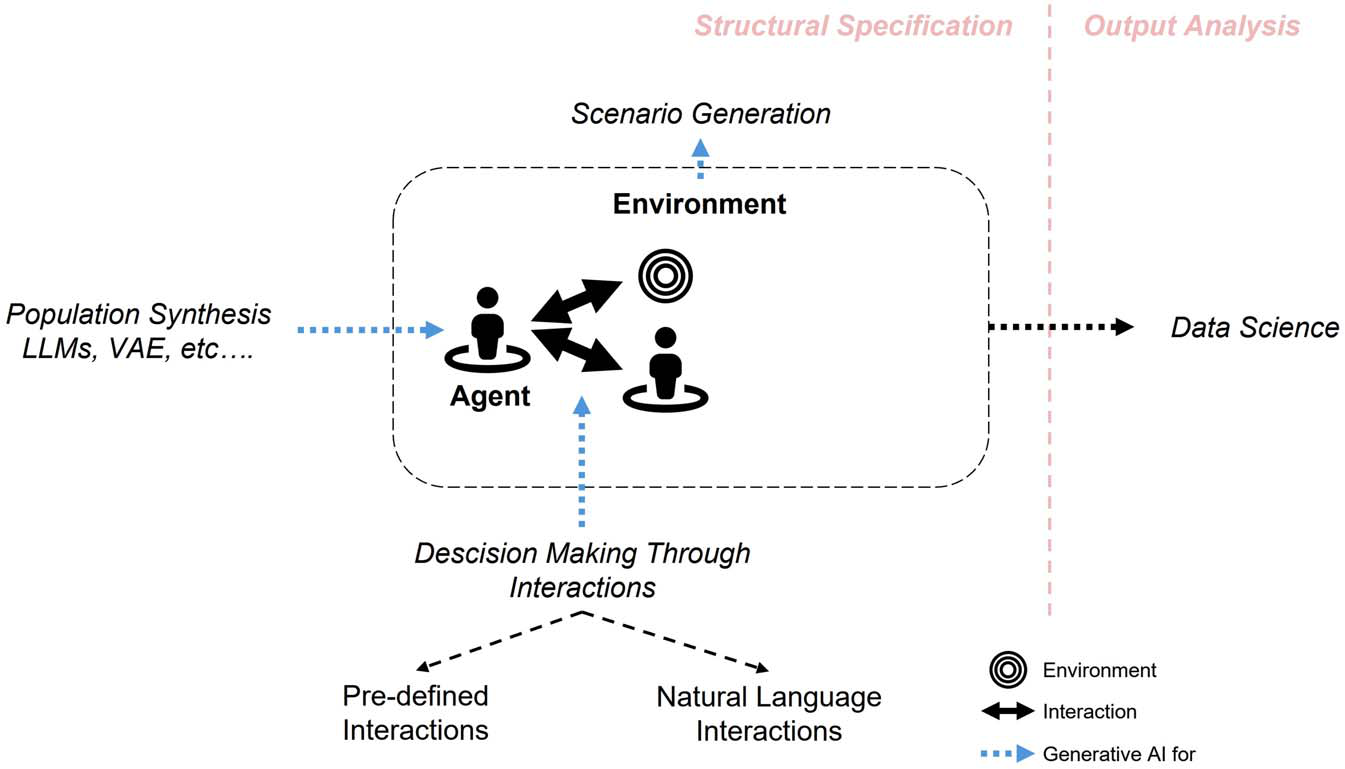
\includegraphics[width=0.95\textwidth,keepaspectratio]{fig1_ai_in_abm.png}
    \caption{AI integration across the two distinct areas of ABM development: Structural Specification and Output Analysis (Source: Base Research Paper Figure 1)}
    \label{fig:fig1_ai_in_abm}
\end{figure}

\subsection{Structural Specification}
Structural specification governs how simulation environments and agent populations are established prior to and during simulation:
\begin{itemize}
    \item \textbf{Population Synthesis:} Generative models create synthetic datasets of agent characteristics, personas and daily activity schedules based on aggregate census data. Crucially, the base paper notes that when generative models generate agents \textit{ex-ante}, it is not accurate to refer to them as GAs, because their within-simulation evolution does not leverage generative processes.
    \item \textbf{Decision Making via Interactions:} Foundation models act as decentralized cognitive engines. Agents perceive environmental states, interpret interactions and formulate behavioral decisions dynamically. Inter-agent communication occurs via open-ended natural language, allowing genuine Generative Agents to emerge.
    \item \textbf{Scenario Generation:} Generative AI synthesizes dynamic environmental perturbations, resource crises and policy shifts without manual scripting.
\end{itemize}

\subsection{Output Analysis}
Output analysis pertains to the interpretation and validation of unfolding simulation states:
\begin{itemize}
    \item \textbf{Macro-Level Emergence Tracking:} Deep learning models monitor high-dimensional simulation state logs, detecting subtle emergent social patterns and collective tipping points.
    \item \textbf{Narrative Summarization and Synthetic Interviewing:} Researchers can directly interview individual agents or synthetic communities in natural language regarding the rationale behind their choices and subjective emotional experiences.
\end{itemize}

\chapter{GENERATIVE AGENTS}
\label{chap:generative_agents}

\section{Formal Architectural Definition}
\label{sec:ga_def}

A Generative Agent is defined as an autonomous computational entity capable of:
\begin{enumerate}[label=\arabic*.]
    \item Perceiving multimodal or natural language sensory streams from its environment;
    \item Maintaining an evolving chronological memory stream of past experiences;
    \item Generating reflective higher-order inferences and abstract beliefs;
    \item Devising and dynamically revising hierarchical plans; and
    \item Communicating with other agents through fluent natural language dialogue.
\end{enumerate}

Architecturally, GABMs decouple simulations into a \textbf{Mechanical Environment Layer} (managing spatial coordinates, collision physics and clock time) and a \textbf{Cognitive Layer} (managing LLM-driven reasoning, memory and dialogue).

\section{Parameters and Status Representation}
\label{sec:parameters_status}

The base research paper establishes a clear distinction between an agent's static parameters and dynamic status:
\begin{itemize}
    \item \textbf{Static Baseline Parameters:} Invariant identity attributes initialized prior to simulation, including demographic data (age, sex, income, occupation), baseline Big Five personality traits and static social network graphs. These are persistent prompts anchoring agent identity.
    \item \textbf{Dynamic Runtime Status:} Fluctuating state variables that evolve during simulation, such as emotional affect, spatial coordinates, active goals and chronological memories, illustrated in Figure~\ref{fig:fig2_feedback_loop}(c).
\end{itemize}

A major practical advantage highlighted in the base paper is that all information contained in the agent status remains in the form of structured text. LLMs can directly interpret, update and reason over structured text without requiring lossy translation into rigid mathematical vectors, facilitating peer-to-peer social influence and dynamic sentiment tracking.

\section{Decision Architectures: Inferential vs. Conversational Loops}
\label{sec:feedback_loops}

\begin{figure}[H]
    \centering
    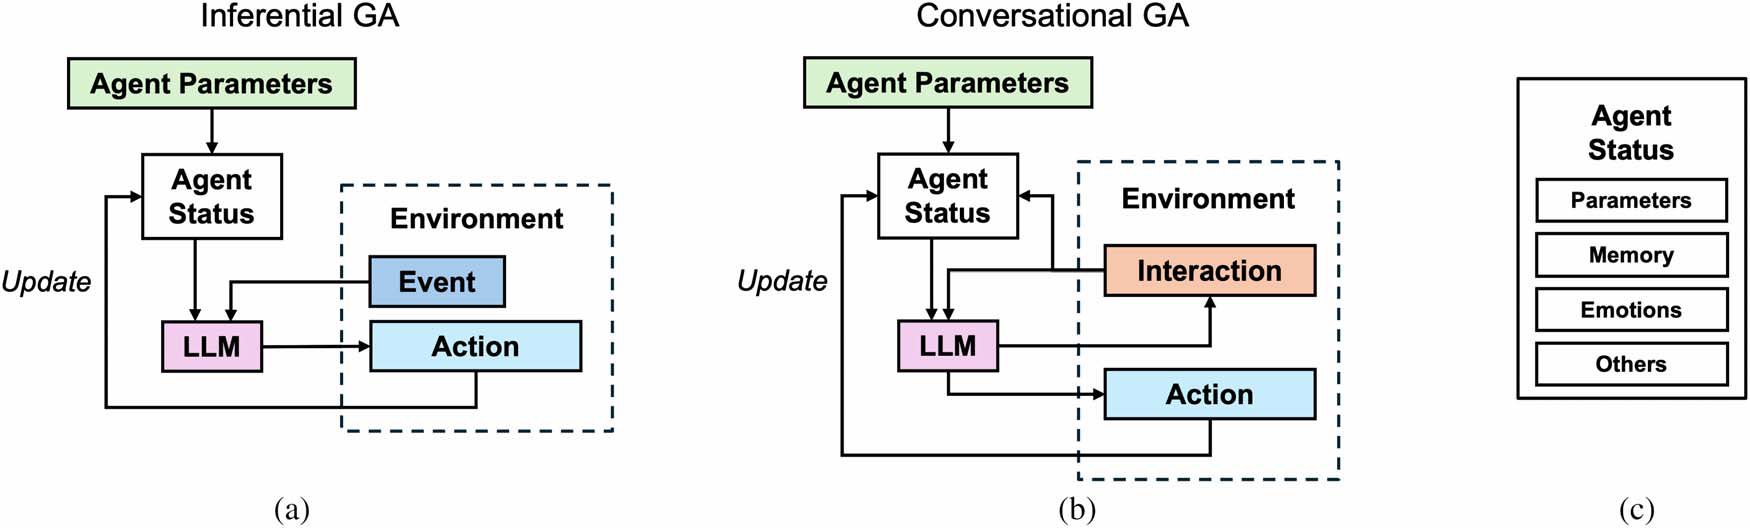
\includegraphics[width=\textwidth,keepaspectratio]{fig2_ga_feedback_loop_status.png}
    \caption{LLM-based feedback loop and status of Generative Agents: (a) Inferential GA feedback loop and (b) Conversational GA feedback loop (Source: Base Research Paper Figure 2)}
    \label{fig:fig2_feedback_loop}
\end{figure}

\begin{enumerate}[label=(\alph*)]
    \item \textbf{Inferential Feedback Loop:} As shown in Figure~\ref{fig:fig2_feedback_loop}(a), the agent ingests its internal status and an environmental event trigger, executes inference and directly outputs a discrete physical action that updates the simulation environment.
    \item \textbf{Conversational Feedback Loop:} As shown in Figure~\ref{fig:fig2_feedback_loop}(b), incoming communicative events trigger an internal status update, prompting the agent to synthesize a natural language response transmitted to neighboring agents.
\end{enumerate}

In grounded environments such as Concordia~\cite{concordia2023}, an explicit Game Master (GM) agent arbitrates interactions, handling world physics, validating physical plausibility and generating event statements.

\section{Core Cognitive Modules}
\label{sec:cognitive_modules}

State-of-the-art generative agents incorporate three core cognitive modules:

\subsection{Memory Stream and Retrieval Scoring}
Agents maintain a chronological database recording all perceptions and actions in natural language strings with timestamps. Because LLM context windows are bounded, relevant memories are retrieved at each step using a linear scoring function:
\begin{equation}
\text{Score}(m, q) = \alpha \cdot \text{Recency}(m) + \beta \cdot \text{Importance}(m) + \gamma \cdot \text{Relevance}(m, q)
\end{equation}
where $\alpha, \beta, \gamma \ge 0$ are non-negative weighting parameters:
\begin{enumerate}[label=\arabic*., itemsep=1pt, parsep=0pt, topsep=2pt]
    \item \textbf{Recency:} Decays exponentially based on elapsed simulation time: $\text{Recency}(m) = e^{-\lambda (t_{\text{current}} - t_{\text{last\_access}})}$ with decay parameter $\lambda > 0$.
    \item \textbf{Importance:} Integer rating from 1 (mundane) to 10 (critical), assigned by the LLM upon memory creation to distinguish trivial events from pivotal occurrences.
    \item \textbf{Relevance:} Cosine similarity between dense embedding vectors of the memory record $\mathbf{e}_m$ and situational query $\mathbf{e}_q$: $\text{Relevance}(m, q) = \frac{\mathbf{e}_m \cdot \mathbf{e}_q}{\|\mathbf{e}_m\| \|\mathbf{e}_q\|}$.
\end{enumerate}

\subsection{Hierarchical Reflection Engine}
To prevent retrieval from becoming flooded with granular observations, the reflection engine periodically synthesizes raw memories into abstract insights. Triggered when cumulative memory importance exceeds a threshold, the agent formulates salient high-level questions, retrieves supporting evidence and stores abstract beliefs back into the stream, creating a hierarchical reflection tree.

\subsection{Dynamic Recursive Planning}
Planning operates recursively: agents draft a broad daily agenda, decompose hourly tasks into 5-to-15 minute action sequences and monitor environmental feedback. If unexpected events occur, execution is interrupted to revise plans dynamically.

\section{Existing GABM Implementations}
\label{sec:prominent_gabms}

\begin{table}[H]
\centering
\vspace{-0.5cm}
\caption{Comparison of existing GABMs, highlighting scenarios, agent characteristics and validation methods}
\label{tab:table2_gabms}
\vspace{0.1cm}
\setlength{\tabcolsep}{3.5pt}
\renewcommand{\arraystretch}{1.05}
\footnotesize
\begin{tabular}{|p{0.8cm}|p{0.8cm}|p{3.8cm}|p{4.2cm}|p{4.4cm}|}
\hline
\textbf{Ref} & \textbf{Year} & \textbf{Framework \& Scenario} & \textbf{Contribution Highlights} & \textbf{Validation Methodology} \\
\hline
\cite{sotopia2024} & 2024 & \textbf{SOTOPIA:} Goal-driven social interactions (cooperation, competition). & Multi-agent benchmark with diverse persona profiles. & Human evaluation vs. LLM-as-a-judge across 7 dimensions. \\
\hline
\cite{socialnorms2024} & 2024 & \textbf{CRSEC:} Social norm emergence in Smallville using 10 GAs. & 4-stage pipeline: Creation, Spreading, Evaluation, Compliance. & 30 human evaluators testing conflict reduction and norm adoption. \\
\hline
\cite{concordia2023} & 2023 & \textbf{Concordia:} Grounded physical and social space. & Modular language agents with centralized Game Master. & Qualitative analysis and design pattern guidelines. \\
\hline
\cite{park2023generative} & 2023 & \textbf{Smallville:} 25 agents in 2D RPG town forming relationships. & Architecture integrating memory stream, reflection, planning. & 100 human evaluators; interview believability scoring. \\
\hline
\cite{s32023} & 2023 & \textbf{S3 Platform:} Social network information diffusion. & LLM agents with attitude and emotion tracking. & Empirical matching against real-world social network traces. \\
\hline
\cite{adornetto2025generative} & 2023 & \textbf{Epidemic GAs:} Emergency dynamics and pandemic decisions. & Inferential GAs for decision-making without conversation. & Visualization verifying alignment with real-world epidemic patterns. \\
\hline
\end{tabular}
\end{table}

Beyond these core platforms, recent architectures introduce key innovations:
\begin{itemize}
    \item \textbf{Lyfe Architecture:} Employs a hierarchical action selection component to delegate only necessary decisions to LLMs, reducing costly API calls while enabling simultaneous conversational interaction with multiple agents.
    \item \textbf{CRSEC Norm Emergence Pipeline:} Implements four modules (Creation \& Representation, Spreading, Evaluation, Compliance) to study normative internalization, demonstrated through an experienced smoker internalizing and enforcing indoor smoking bans.
    \item \textbf{Qualitative Emotion Simulation:} The S3 platform tracks dynamic attitudes and three-tier emotional intensity levels (calm, moderate, intense) during information propagation following real-world societal shocks.
    \item \textbf{Urban GABM Extensions:} Incorporates commuter adaptation under transit disruptions and extreme weather, alongside socioeconomic neighborhood evolution assessing affordable housing policies.
\end{itemize}

\chapter{INFORMAL THEORY OF ABMS VALIDATION}
\label{chap:abm_validation}

\section{Epistemological Principles of Simulation Validation}
\label{sec:validation_principles}

Validation in computational modeling establishes whether a computational model accurately represents the target real-world system within its intended domain~\cite{grimm2006standard}. Traditional modeling literature draws a fundamental distinction between:
\begin{enumerate}[label=\arabic*.]
    \item \textbf{Verification:} An internal algorithmic and engineering check answering the question: \textit{``Was the model built right?''} Verification ensures that software code, state transition logic and numerical algorithms correctly implement conceptual specifications without programming flaws.
    \item \textbf{Validation:} An external empirical evaluation answering the question: \textit{``Was the right model built?''} Validation assesses whether simulated behaviors faithfully correspond to empirical real-world observations and physical ground truth.
\end{enumerate}

The base research paper highlights the four-step validation guidelines formulated by Rand and Rust~\cite{adornetto2025generative}. Steps 1 and 2 focus on empirical validation: Step~1 evaluates input parameters against real-world data, while Step~2 statistically validates model outputs against empirical observations or comparable benchmarks. Steps 3 and 4 encompass face validation: Step~3 conducts microface validation of individual-level mechanisms, and Step~4 performs macroface validation of aggregate emergent patterns.

\section{Foundational Validation Methodologies}
\label{sec:foundational_val}

Traditional ABM validation relies on five established foundational methods:
\begin{enumerate}[label=\arabic*.]
    \item \textbf{Data Analytics:} Quantitative statistical comparison of simulated outputs with historical measurements using goodness-of-fit tests, regression residuals and distribution tests (e.g., Kolmogorov-Smirnov).
    \item \textbf{Model Docking (Alignment):} Comparing two independent simulation models developed with distinct software architectures calibrated against identical input benchmarks to verify that emergent behaviors are genuine systemic properties rather than software artifacts.
    \item \textbf{Empirical Validation:} Initializing simulations with historical conditions from time $t_0$ and evaluating predictive accuracy against observed ground truth up to time $t_1$.
    \item \textbf{Sampling Techniques:} Parameter space exploration via Latin Hypercube Sampling (LHS) and Monte Carlo sweeps to evaluate stability and identify sensitivity thresholds across high-dimensional parameter spaces.
    \item \textbf{Visualization:} Graphical displays to detect anomalies in emergent spatial distributions and temporal trajectory patterns.
\end{enumerate}

\section{Advanced Analytical Validation Methods}
\label{sec:advanced_val}

Advanced validation frameworks incorporate analytical methods to address noisy or limited data:
\begin{itemize}
    \item \textbf{Bootstrapping:} Non-parametric resampling of model output data to establish empirical confidence intervals and evaluate robustness without restrictive distributional assumptions.
    \item \textbf{Causal Analysis:} Directed Acyclic Graphs (DAGs) and counterfactual intervention testing to differentiate genuine causal mechanisms from spurious statistical correlations.
    \item \textbf{Inverse Generative Social Science (IGSS):} Using genetic programming and evolutionary search algorithms to explore potential agent behavioral rules, backtracking from macro-patterns to discover the minimal micro-mechanisms capable of generating target social phenomena.
    \item \textbf{Spatial Analytics:} Spatial statistics, such as Moran's $I$ and point pattern spatial analysis, to validate simulated geographic distributions against empirical GIS datasets.
\end{itemize}

In urban traffic simulations, these methods operate cohesively: empirical validation verifies traffic counts against road sensors, visualization monitors queue formation, sampling tests sensitivity to driver reaction times and causal analysis isolates the structural root causes of congestion bottlenecks.

\section{Empirical and Face Validation Dimensions}
\label{sec:empirical_face}

In social simulations where quantitative ground truth is sparse, researchers rely on \textbf{Face Validation} to assess behavioral credibility based on expert domain knowledge~\cite{adornetto2025generative}:
\begin{enumerate}[label=\arabic*.]
    \item \textbf{Microface Validation:} Evaluates individual agent actions and internal decision logic against established psychological, cognitive and behavioral theories.
    \item \textbf{Macroface Validation:} Assesses whether aggregate population distributions and emergent systemic patterns correspond to real-world social phenomena.
    \item \textbf{Face Validation Methodologies:} As formalized by Kl{\"u}gl, face validation incorporates three distinct assessment elements:
    \begin{itemize}
        \item \textit{Animation Assessment:} Experts review real-time simulation animations to ensure pedestrian flows, vehicle queues and localized interactions appear realistic.
        \item \textit{Output Assessment:} Human experts evaluate simulation outputs for plausibility. This process can be automated when input-output relationships are formally defined via constraints and rules.
        \item \textit{Immersive Assessment:} Validators immerse themselves within the simulation by adopting the perspective of an individual agent (potentially via Virtual Reality interfaces) to evaluate behavioral plausibility, emotional responses and interpersonal dynamics firsthand when empirical data is unavailable.
    \end{itemize}
\end{enumerate}

\chapter{GABMS VALIDATION}
\label{chap:gabms_validation}

\section{The Fundamental Validation Dilemma}
\label{sec:black_box_dilemma}

The integration of LLMs introduces the \textbf{Fundamental Validation Dilemma}. While traditional ABMs are transparent white-box systems with deterministic state transitions, Generative Agents rely on foundation models that function as probabilistic black boxes:
\begin{enumerate}[label=\arabic*.]
    \item \textbf{Stochastic Non-Determinism:} Temperature decoding and probabilistic sampling generate divergent paths from identical starting seeds, invalidating deterministic unit tests.
    \item \textbf{Opaque Internal Reasoning:} Internal states are distributed across billions of continuous parameters without explicit algebraic transition equations.
    \item \textbf{High-Dimensional Output Spaces:} Agent actions include unconstrained natural language dialogues requiring qualitative evaluation of semantic coherence, emotional nuance and truthfulness.
\end{enumerate}

\section{GABM Validation Workflows}
\label{sec:validation_workflows}

Figure~\ref{fig:fig3_validation_workflows} illustrates the integrated validation architecture formulated in the base paper, connecting validation methods with distinct validation purposes.

\begin{figure}[H]
    \centering
    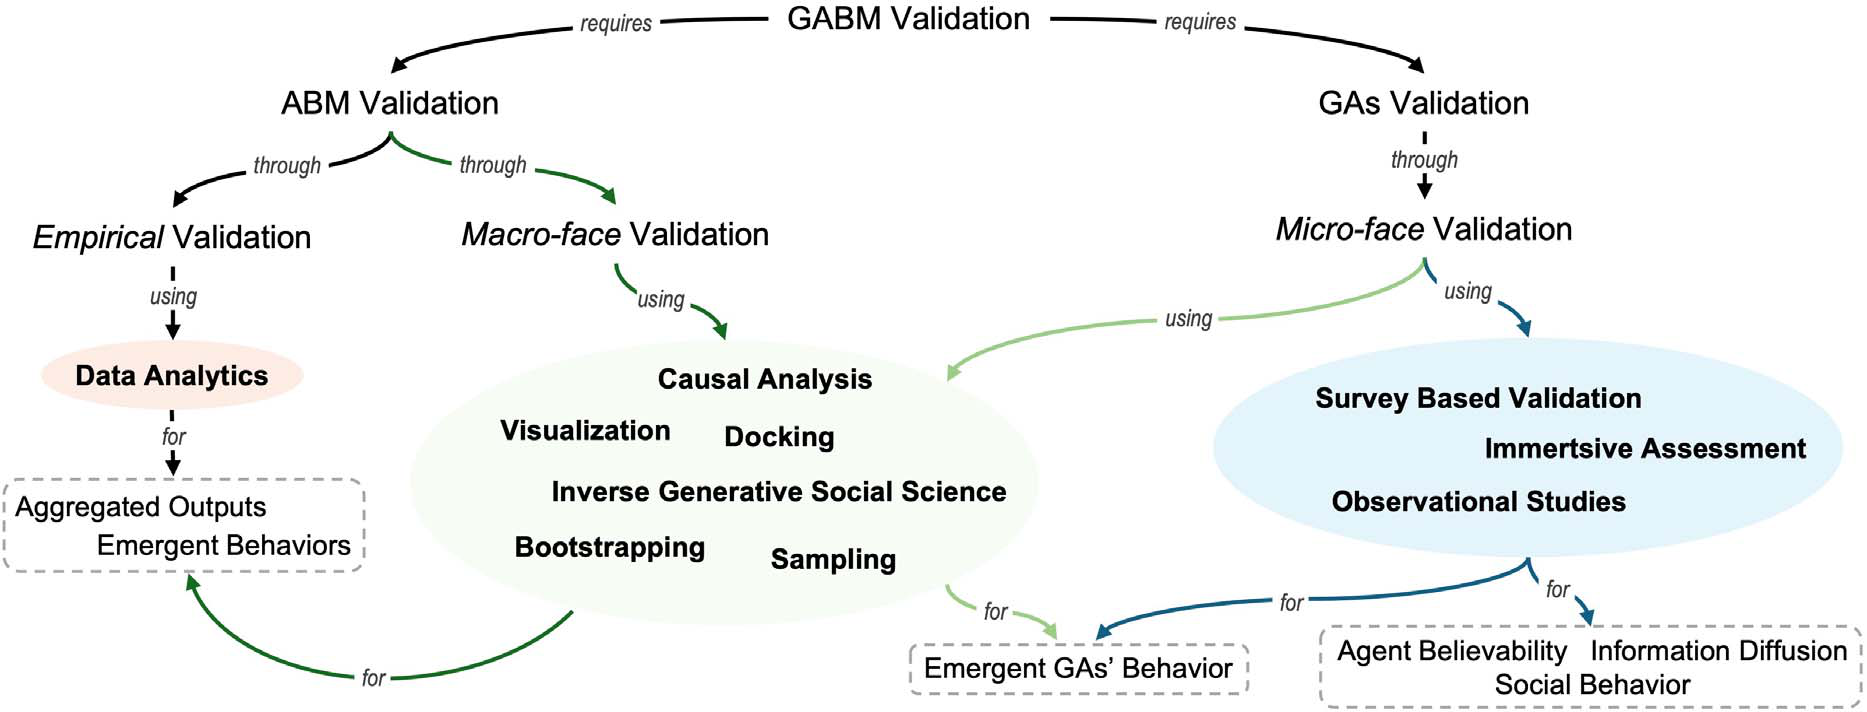
\includegraphics[width=\textwidth,keepaspectratio]{fig3_gabm_validation_workflows.png}
    \caption{Validation workflows for GABMs, illustrating how various validation methods align with distinct validation purposes (Source: Base Research Paper Figure 3)}
    \label{fig:fig3_validation_workflows}
\end{figure}

The framework operates across three distinct pathways that are given below.
\begin{enumerate}[label=\arabic*.]
    \item \textbf{Empirical Pathway:} Uses micro-level data (census, demographics) to condition baseline parameters and macro-level data (traffic counts, voting outcomes) to evaluate aggregate simulation trajectories statistically.
    \item \textbf{Macroface Pathway:} Validates collective emergent phenomena (social network topologies, norm adoption rates, spatial clustering) that arise spontaneously without centralized coordination.
    \item \textbf{Microface Pathway:} Assesses individual agent plausibility via structured interviews, ablation testing and automated dialogue audits.
\end{enumerate}

\section{Validating Existing Generative Agent Implementations}
\label{sec:human_eval_studies}

Validation methodologies across existing GABM platforms combine human and automated protocols:
\begin{itemize}
    \item \textbf{Smallville Evaluation Protocols:} In the \textit{Ablation Study}, 100 human evaluators scored agent responses across self-knowledge, memory retrieval, planning consistency, reaction plausibility and reflection depth, confirming the full architecture achieves superior believability over ablated baselines. In the \textit{End-to-End Evaluation}, a two-day simulation tracked information diffusion regarding a Valentine's Day party and mayoral candidacy, measuring social network density over time and agent party attendance.
    \item \textbf{Concordia Validation Framework:} Formulates the \textit{Similarity Principle}, asserting that testing one prediction provides confidence in related predictions within a behavioral family. Emphasizes direct measurement on held-out test data as the gold standard, alongside \textit{Algorithmic Fidelity} to condition agents on socio-demographic backstories for hard-to-reach populations.
    \item \textbf{S3 Platform Empirical Validation:} Validates online social network simulations against empirical event traces across information dissemination curves, three-tier emotional dynamics (calm, moderate, intense) and interactive behaviors (forward, create, inactive) evaluated via Accuracy, AUC and F1-score.
    \item \textbf{SOTOPIA-EVAL Benchmark:} Evaluates goal-driven interactions across seven dimensions: Goal Completion, Believability, Knowledge Gained, Secret Keeping, Relationship Dynamics, Social Norms and Financial Benefit. Dual human and GPT-4 evaluations reveal high agreement on objective metrics, but show limitations in evaluating subtle social norms and secret-keeping.
\end{itemize}

\section{Automated Validation: LLM-as-a-Judge and Algorithmic Fidelity}
\label{sec:llm_as_judge}

To address human evaluation expense, researchers utilize \textbf{LLM-as-a-Judge}~\cite{zheng2023judging}, prompting foundation models to score multi-agent interactions across structured rubrics. While automated judges offer scalability, they exhibit nuance blindness regarding sarcasm, passive aggression and deception, alongside an evaluator self-preference bias toward models from their own architectural family.

Consequently, the base paper emphasizes \textbf{Algorithmic Fidelity}~\cite{argyle2023out}. Before deploying LLMs as simulation agents or evaluators, researchers must benchmark baseline persona profiles against validated sociological surveys~\cite{serapio2023personality} to detect and mitigate systemic cultural, political and demographic biases.

\chapter{ABM VS GABM: A COMPARISON}
\label{chap:abm_vs_gabm}

\section{Systematic Comparative Dimensions}
\label{sec:comp_dimensions}

\begin{table}[H]
\centering
\vspace{-0.5cm}
\caption{Comparison between traditional ABM paradigms and Generative ABM (GABM)}
\label{tab:table3_comparison}
\vspace{0.2cm}
\setlength{\tabcolsep}{4pt}
\renewcommand{\arraystretch}{1.15}
\small
\begin{tabular}{|p{5.4cm}|p{2.2cm}|p{2.2cm}|p{2.2cm}|p{2.2cm}|}
\hline
\textbf{Evaluation Dimension} & \textbf{Rule-based} & \textbf{EA-based} & \textbf{RL-based} & \textbf{GABM} \\
\hline
\multicolumn{5}{|l|}{\textbf{1. Resources}} \\
\hline
\quad Computational Efficiency & Advantage & Limitation & Limitation & Limitation \\
\hline
\quad Scalability & Advantage & Limitation & Limitation & Limitation \\
\hline
\quad Data or Domain-Specific Knowledge & Advantage & Advantage & Advantage & Advantage \\
\hline
\multicolumn{5}{|l|}{\textbf{2. Agent Design}} \\
\hline
\quad Control over Agents & Advantage & Limitation & Limitation & Limitation \\
\hline
\quad Learning During Simulation & Limitation & Advantage & Advantage & Limitation \\
\hline
\quad Real-Time Optimization & Limitation & Advantage & Advantage & Limitation \\
\hline
\quad Hyperparameters Tuning & Advantage & Limitation & Limitation & Limitation \\
\hline
\quad Fast Prototyping & Limitation & Limitation & Limitation & Advantage \\
\hline
\multicolumn{5}{|l|}{\textbf{3. Agent Behavior}} \\
\hline
\quad Determinism & Advantage & Limitation & Limitation & Limitation \\
\hline
\quad Reliable Decision-Making & Advantage & Limitation & Limitation & Limitation \\
\hline
\quad Evolution & Limitation & Advantage & Advantage & Limitation \\
\hline
\quad Cognitive Functions Simulation & Limitation & Limitation & Limitation & Advantage \\
\hline
\quad Language Human-like Interactions & Limitation & Limitation & Limitation & Advantage \\
\hline
\quad Flexible and Reactive Decisions & Limitation & Limitation & Advantage & Advantage \\
\hline
\quad Nuanced Mental Models & Limitation & Limitation & Limitation & Advantage \\
\hline
\multicolumn{5}{|l|}{\textbf{4. Validation}} \\
\hline
\quad Transparency of Decision-Making & Advantage & Limitation & Limitation & Limitation \\
\hline
\quad Validation Efficiency & Advantage & Limitation & Limitation & Limitation \\
\hline
\quad Direct Human-Agent Interaction & Limitation & Limitation & Limitation & Advantage \\
\hline
\end{tabular}
\end{table}

Table~\ref{tab:table3_comparison} reproduces the comparative analysis from Table III of the base paper, contrasting traditional ABMs (Rule-based, EA-based, RL-based) with GABMs across Resources, Agent Design, Agent Behavior and Validation.

\section{Key Trade-Offs and Architectural Insights}
\label{sec:trade_offs}

\subsection{Resources: Efficiency, Scalability and Knowledge}
Rule-based models require simple CPU arithmetic ($\mathcal{O}(1)$ time complexity), scaling to millions of agents in macroeconomic or epidemic models. GABMs incur significant GPU inference latency and token costs, restricting cohorts to dozens or hundreds of agents. However, GABMs leverage broad pretrained world knowledge, eliminating the need to construct explicit domain rules from scratch.

\subsection{Agent Design: Control, Learning and Prototyping}
Rule-based models provide deterministic control over every logic branch. GABMs rely on prompt engineering, which is susceptible to semantic drift. Furthermore, LLM weights remain frozen during simulation; agent learning is confined to in-context memory accumulation. However, GABMs provide superior \textbf{Fast Prototyping}, allowing complex personas to be defined in minutes via natural language.

\subsection{Behavior and Validation: Cognitive Fidelity vs. Transparency}
Rule-based systems offer mathematical transparency and replicability, but cannot model open-ended language, emotional states or mental models. GABMs excel in cognitive realism and introduce \textbf{Direct Human-Agent Interaction}, enabling researchers to interview agents regarding their motivations.

\section{Complementarity and Methodological Synthesis}
\label{sec:complementarity}

The core conclusion of the comparative analysis in the base paper is that traditional ABMs and GABMs are complementary rather than mutually exclusive. Traditional ABMs contribute computational efficiency, deterministic control and demographic scalability; GABMs contribute cognitive realism, linguistic communication and adaptive reasoning. Effective simulation requires hybrid methodologies that combine the advantages of both paradigms.

%=========================================================
% CHAPTER 8: GABMS: EMERGING CHALLENGES
%=========================================================

\chapter{GABMS: EMERGING CHALLENGES}
\label{chap:emerging_challenges}

\section{Challenge 1: Large Language Model Hallucinations}
\label{sec:hallucinations}

Hallucinations undermine GABM validity across two primary modes:
\begin{enumerate}[label=\arabic*.]
    \item \textbf{Factuality Hallucinations:} Generating assertions that contradict objective environmental ground truth, such as asserting a bridge crosses an uncrossable river, navigating impassable obstacles or fabricating physical objects that do not exist within the simulation state space. Unlike generic NLP where hallucinations merely produce inaccurate text, in an ABM hallucinated physical actions propagate through the environmental feedback loop, permanently corrupting spatial consistency.
    \item \textbf{Faithfulness Hallucinations:} Violating assigned persona constraints, moral values or historical context, such as an assigned pacifist initiating unprovoked violent conflict or a historical persona using contemporary technical jargon. In social simulations, faithfulness errors invalidate persona conditioning and destroy demographic representativeness.
\end{enumerate}

Mitigation strategies operate across three systematic stages:
\begin{itemize}
    \item \textbf{Data Stage:} Grounding prompts via Retrieval-Augmented Generation (RAG) using verified real-time simulation facts and environment state logs to anchor agent context.
    \item \textbf{Training Stage:} Applying sensitive neuron dropout, domain-specific instruction tuning and RLHF to enforce persona consistency and penalize behavioral drift.
    \item \textbf{Inference Stage:} Enforcing formal grammar constraints (e.g., JSON schema, context-free grammars) and deploying peer verification protocols where secondary agents audit and cross-verify behavioral outputs.
\end{itemize}

\section{Challenge 2: Validation Bottlenecks and Nuance Detection}
\label{sec:val_bottlenecks}

Automated LLM judges exhibit critical limitations that impede robust evaluation:
\begin{enumerate}[label=\arabic*.]
    \item \textbf{Nuance Blindness:} Evaluators struggle with passive aggression, sarcasm, humor and strategic deception, showing systematic bias toward artificially polite or sycophantic agents.
    \item \textbf{Evaluator Self-Preference Bias:} Foundation models consistently assign higher scores to responses generated by models belonging to their own architectural family, creating circular evaluation loops.
    \item \textbf{Lack of Standardized Benchmarks:} Absence of standardized multi-agent simulation benchmarks and open datasets prevents rigorous cross-study comparability and reproducibility.
\end{enumerate}

\section{Challenge 3: Computational Overhead and Scaling Bottlenecks}
\label{sec:comp_bottlenecks}

Scaling constraints arise across three interrelated computational bottlenecks:
\begin{enumerate}[label=\arabic*.]
    \item \textbf{Quadratic Self-Attention Overhead:} Computational complexity scales quadratically with prompt token length $n$~\cite{vaswani2017attention}:
    \begin{equation}
    \text{Complexity}_{\text{Attention}} = \mathcal{O}(n^2 \cdot d)
    \end{equation}
    where $d$ is embedding dimension. As simulation history expands, memory streams lengthen prompts, escalating GPU memory bandwidth demands and inference latency.
    \item \textbf{Pairwise Communication Scaling:} In a network of $N$ interacting agents, potential dialogue channels scale quadratically:
    \begin{equation}
    \text{Complexity}_{\text{Communication}} = \mathcal{O}(N^2)
    \end{equation}
    requiring substantial inference calls per simulation tick in decentralized communication networks.
    \item \textbf{Memory Retrieval Indexing:} Vector search across $M$ records introduces indexing complexity $\mathcal{O}(\log M)$ to $\mathcal{O}(M)$ per agent per tick, accompanied by substantial commercial API financial costs during extended simulation runs.
\end{enumerate}

\chapter{DISCUSSION}
\label{chap:discussion}

\section{Addressing Broader Epistemological Questions}
\label{sec:epist_questions}

The base research paper examines foundational epistemological questions driving social simulation:
\begin{enumerate}[label=\arabic*.]
    \item \textbf{Macroscopic Pattern Emergence:} How macro-patterns emerge from micro-interactions with diverse, personality-driven agents.
    \item \textbf{Information and Innovation Diffusion:} How ideas spread dynamically through curious, skeptical and communicative agents.
    \item \textbf{Strategic Adaptation in Dynamic Environments:} How agents modify strategies autonomously in resource-limited game settings.
    \item \textbf{Social Network Influence and Polarization:} How interpersonal persuasion and conformity shape echo chambers and polarization.
    \item \textbf{Linguistic and Framing Biases:} How natural language framing influences social deliberation and consensus formation.
\end{enumerate}

The base paper addresses Epstein's classic epistemological challenge: does generating a social pattern with an opaque neural network constitute a scientific explanation? Explanatory power is established through mechanistic interpretability and prompt perturbation testing, verifying which persona attributes or normative beliefs were necessary and sufficient to drive emergent outcomes. Furthermore, GABMs capture subjective human experiences: in traffic simulations, route choices are driven by emotional triggers (avoiding fear-inducing routes or choosing scenic paths) rather than pure shortest-path heuristics. In data-sparse domains, such as disaster emergency scenarios or informal settlements, GABMs facilitate rich qualitative analyses of social dynamics where sensor infrastructure is unavailable.

\section{Cities: A Natural Testbed for GABMs}
\label{sec:cities_testbed}

Urban environments provide an ideal deployment testbed:
\begin{itemize}
    \item \textbf{Textual Alignment:} Urban regulations, historical archives, transportation policies and census data align closely with LLM training corpora, providing rich baseline representations.
    \item \textbf{Qualitative Experience Mapping (QEM):} Traditional models (such as MATSim~\cite{matsim2016}) simulate physical trajectories. GABMs enable tracking subjective experiences: safety perceptions in unlit corridors, park aesthetic appreciation and transit stress, informing human-centric urban design and responsive policy-making.
\end{itemize}

\section{The Proposed Paradigm: Combined Hybrid ABM-GABM Architecture}
\label{sec:hybrid_architecture}

To overcome computational bottlenecks while preserving behavioral realism, the base paper proposes an integrated \textbf{Hybrid ABM-GABM Architecture}:
\begin{enumerate}[label=\arabic*.]
    \item \textbf{Mechanistic Layer (Traditional ABM):} High-frequency, deterministic processes (kinematics, collision avoidance, obstacle navigation, shortest-path routing) execute at $\mathcal{O}(1)$ or $\mathcal{O}(N)$ without invoking LLMs.
    \item \textbf{Cognitive Layer (Generative Agents):} Foundation model inference is invoked selectively only for complex deliberations, ethical dilemmas and social dialogue.
\end{enumerate}

\subsection{Case Study: Building Fire Evacuation}
In an emergency building fire evacuation, the mechanistic layer computes toxic smoke dispersion and obstacle navigation via cellular automata, while the generative cognitive layer evaluates moral dilemmas, such as deciding whether to re-enter a hazard area to rescue a trapped colleague versus immediate egress. In urban land-use simulations, hybrid validation couples sensor data analytics for crowd density with agent interviews to examine why individuals alter travel modes or avoid overcrowded transit hubs.

\chapter{CONCLUSION}
\label{chap:conclusion}

\section{Summary of Key Technical Insights}
\label{sec:conclusion_summary}

This seminar report has conducted an in-depth technical investigation into the paradigm of Generative Agents in Agent-Based Modeling, based on the comprehensive survey paper by Adornetto et al.~published in \textit{IEEE Transactions on Artificial Intelligence} (December 2025). The introduction of foundation models into agent-based modeling marks a decisive departure from neoclassical assumptions of perfect rationality (\textit{homo economicus}) toward heterogeneous, cognitively plausible human simulacra. By embedding large language models into agent architectures through episodic memory streams, associative retrieval scoring, hierarchical reflection trees and dynamic recursive planning, generative agents demonstrate remarkable autonomy, believable social interactions and spontaneous normative emergence.

A foundational insight emphasized throughout this work is the epistemological clarification distinguishing classical generative social science from technological generative artificial intelligence. Joshua Epstein's seminal principle established that a social phenomenon is explained if and only if it can be grown computationally from decentralized local interactions. The presence of generative artificial intelligence is not in itself sufficient to establish generative social science; rather, true explanatory power depends on modeling the internal behavioral mechanisms that give rise to macro-level regularities. Generative Agent-Based Models unite these two paradigms, leveraging language models to empower individual agent deliberation while preserving the bottom-up explanatory ethos of agent-based modeling.

The comparative analysis across resources, agent design, agent behavior and validation establishes that traditional ABMs and GABMs represent complementary rather than mutually exclusive methodologies. Traditional rule-based and evolutionary models provide computational efficiency, deterministic reproducibility and demographic scalability to millions of agents. In contrast, GABMs provide cognitive nuance, natural language communication and rapid persona prototyping. To address the black-box validation dilemma arising from opaque neural architectures, researchers have established multi-tiered validation workflows that combine quantitative empirical data analytics, qualitative face validation, human interview audits and automated LLM-as-a-Judge evaluations calibrated by algorithmic fidelity. The combined hybrid ABM-GABM architecture bridges these methodologies, coupling high-frequency deterministic physics engines with selective cognitive language model deliberation to achieve both computational tractability and behavioral authenticity.

\section{Future Research Trajectories}
\label{sec:conclusion_future}

Future research in Generative Agent-Based Modeling must address several critical frontiers to enable widespread adoption in academic and policy domains. A primary imperative is the development of specialized Small Language Models (SLMs) and parameter-efficient architectures. Deploying compact, on-device models fine-tuned specifically for social reasoning will substantially reduce self-attention latency, lower hardware memory demands and eliminate dependency on costly cloud API services during large-scale simulations.

Simultaneously, the computational social science community must establish standardized, open-source simulation benchmarks and shared evaluation datasets. Similar to established benchmarks in natural language processing and computer vision, standardized multi-agent environments will enable rigorous cross-study comparisons, allowing researchers to evaluate competing cognitive architectures across uniform social tasks, normative emergence scenarios and collective action dilemmas.

Rigorous mathematical frameworks must also be established to formulate formal upper bounds on hallucination probabilities within policy-critical simulations. As generative models are increasingly applied to municipal transit planning, public health protocols and socioeconomic modeling, developing constrained decoding formalisms and multi-agent peer verification protocols will be essential to ensure synthetic agents adhere strictly to environmental ground truth and assigned demographic profiles.

Finally, the expanding cognitive capabilities of generative agents necessitate the formulation of robust ethical guidelines and governance frameworks. Researchers must institute systematic algorithmic fidelity audits to prevent the unexamined propagation of cultural, demographic and socioeconomic biases inherited from foundation model pretraining corpora. Establishing rigorous ethical boundaries will ensure that generative agent simulations serve as reliable, equitable and transparent instruments for investigating complex human societies.

%=========================================================
% REFERENCES (UNNUMBERED HEADING)
%=========================================================

\chapter*{References}
\label{chap:references}
\addcontentsline{toc}{chapter}{References}

\begingroup
\fontsize{11}{14}\selectfont
\setlength{\parskip}{0pt}
\begin{enumerate}[label={[\arabic*]}, itemsep=2pt, parsep=0pt, topsep=0pt, leftmargin=2em]

\bibitem{adornetto2025generative}
C.~Adornetto, A.~Mora, K.~Hu, L.~I.~Garcia, P.~Atchade-Adelomou, G.~Greco, L.~A.~A.~Pastor and K.~Larson,
``Generative Agents in Agent-Based Modeling: Overview, Validation and Emerging Challenges,''
\textit{IEEE Transactions on Artificial Intelligence}, vol.~6, no.~12, pp.~3165-3184, Dec.~2025, doi: 10.1109/TAI.2025.3566362.

\bibitem{park2023generative}
J.~S.~Park, J.~C.~O'Brien, C.~J.~Cai, M.~R.~Morris, P.~Liang and M.~S.~Bernstein,
``Generative Agents: Interactive Simulacra of Human Behavior,''
in \textit{Proc. 36th Annual ACM Symposium on User Interface Software and Technology (UIST)}, San Francisco, CA, USA, Oct.~2023, pp.~1-22.

\bibitem{schelling1971dynamic}
T.~C.~Schelling,
``Dynamic Models of Segregation,''
\textit{Journal of Mathematical Sociology}, vol.~1, no.~2, pp.~143-186, 1971.

\bibitem{epstein1999generative}
J.~M.~Epstein,
``Agent-Based Computational Models and Generative Social Science,''
\textit{Complexity}, vol.~4, no.~5, pp.~41-60, May/Jun.~1999.

\bibitem{reynolds1987flocks}
C.~W.~Reynolds,
``Flocks, Herds and Schools: A Distributed Behavioral Model,''
in \textit{Proc. 14th Annual Conference on Computer Graphics and Interactive Techniques (SIGGRAPH)}, Anaheim, CA, USA, Aug.~1987, pp.~25-34.

\bibitem{holland1992adaptation}
J.~H.~Holland,
\textit{Adaptation in Natural and Artificial Systems: An Introductory Analysis with Applications to Biology, Control and Artificial Intelligence},
Cambridge, MA, USA: MIT Press, 1992.

\bibitem{sutton2018reinforcement}
R.~S.~Sutton and A.~G.~Barto,
\textit{Reinforcement Learning: An Introduction},
2nd~ed., Cambridge, MA, USA: MIT Press, 2018.

\bibitem{sotopia2024}
H.~Wang, X.~Guo, Z.~Deng, H.~Shi, H.~Shen, B.~Zheng, E.~P.~Xing and Z.~Hu,
``Sotopia: Interactive Evaluation for Social Intelligence in Language Agents,''
in \textit{Proc. International Conference on Learning Representations (ICLR)}, Vienna, Austria, May~2024.

\bibitem{socialnorms2024}
S.~He, H.~Zheng, L.~Du and W.~Ding,
``Emergence of Social Norms in Generative Agent Societies: Principles and Architecture,''
in \textit{Proc. 38th AAAI Conference on Artificial Intelligence (AAAI)}, Vancouver, Canada, Feb.~2024, pp.~22120-22128.

\bibitem{concordia2023}
A.~Vezhnevets, J.~P.~Agapiou, A.~Aharon, R.~Boning, E.~A.~Duenez-Guzman, J.~Leibo, et~al.,
``Generative Agent-Based Modeling with Actions Grounded in Physical, Social or Digital Space Using Concordia,''
\textit{arXiv preprint arXiv:2312.03664}, Dec.~2023.

\bibitem{s32023}
C.~Gao, X.~Lan, Z.~Lu, J.~Mao, J.~Piao, H.~Wang, D.~Jin and Y.~Li,
``S$^3$: Social-Network Simulation System with Large Language Model-Empowered Agents,''
\textit{arXiv preprint arXiv:2307.14984}, Jul.~2023.

\bibitem{vaswani2017attention}
A.~Vaswani, N.~Shazeer, N.~Parmar, J.~Uszkoreit, L.~Jones, A.~N.~Gomez, L.~Kaiser and I.~Polosukhin,
``Attention Is All You Need,''
in \textit{Advances in Neural Information Processing Systems (NeurIPS)}, Long Beach, CA, USA, Dec.~2017, pp.~5998-6008.

\bibitem{argyle2023out}
L.~P.~Argyle, E.~C.~Busby, N.~Fulda, J.~R.~Gubler, C.~Rytting and D.~Wingate,
``Out of One, Many: Using Language Models to Simulate Human Samples,''
\textit{Political Analysis}, vol.~31, no.~3, pp.~337-351, Jul.~2023.

\bibitem{axtell2002why}
R.~Axtell,
``Why Agents? On the Varied Motivations for Agent Computing in the Social Sciences,''
in \textit{Proc. Workshop on Agent-Based Modeling: Investment, Risk and Policy}, Santa Fe Institute, Santa Fe, NM, USA, 2002.

\bibitem{bonabeau2002agent}
E.~Bonabeau,
``Agent-Based Modeling: Methods and Techniques for Simulating Human Systems,''
\textit{Proc. National Academy of Sciences (PNAS)}, vol.~99, no.~suppl.~3, pp.~7280-7287, May~2002.

\bibitem{macal2010tutorial}
C.~M.~Macal and M.~J.~North,
``Tutorial on Agent-Based Modelling and Simulation,''
\textit{Journal of Simulation}, vol.~4, no.~3, pp.~151-162, Sep.~2010.

\bibitem{grimm2006standard}
V.~Grimm, U.~Berger, F.~Bastiansen, S.~Eliassen, V.~Ginot, J.~Giske, et~al.,
``A Standard Protocol for Describing Individual-Based and Agent-Based Models,''
\textit{Ecological Modelling}, vol.~198, no.~1-2, pp.~115-126, Sep.~2006.

\bibitem{matsim2016}
A.~Horni, K.~Nagel and K.~W.~Axhausen,
\textit{The Multi-Agent Transport Simulation MATSim},
London, UK: Ubiquity Press, 2016.

\bibitem{serapio2023personality}
G.~Serapio-Garcia, M.~Mustafa, S.~Verma, M.~Caron, M.~Matari{\'c} and A.~Faust,
``Personality Traits in Large Language Models,''
\textit{arXiv preprint arXiv:2307.00184}, Jul.~2023.

\bibitem{zheng2023judging}
L.~Zheng, W.~Chiang, Y.~Sheng, S.~Zhuang, Z.~Wu, Y.~Zhuang, Z.~Lin, Z.~Li, D.~Xing, H.~Zhang, J.~E.~Gonzalez and I.~Stoica,
``Judging LLM-as-a-Judge with MT-Bench and Chatbot Arena,''
in \textit{Advances in Neural Information Processing Systems (NeurIPS)}, New Orleans, LA, USA, Dec.~2023, pp.~46595-46623.

\end{enumerate}
\endgroup

\end{document}